
%--------------- Personalize your document here ---------------

\author{Ths.Dương Hữu Phúc} % Enter your name
\newcommand{\studentID}{Student ID} % enter your student ID
\newcommand{\supervisorone}{Nguyễn Thành Khang - 518H0372} % Enter your supervisor's name
\newcommand{\supervisortwo}{Ngô Văn Quang Trường - 518H0073}% Leave it empty or enter your second supervisor's name 
\newcommand{\department}{Phát triển hệ thống thông tin doanh nghiệp}
\newcommand{\exam}{HAPPY TOUR}
\newcommand{\K}{Khóa:K22}

\date{Tp.Hồ Chí Minh, 2021} % insert a specific date	


\documentclass[a4paper,12pt]{article}
\usepackage[left=30mm,top=30mm,right=30mm,bottom=30mm]{geometry}
\usepackage{etoolbox} %required for cover page
\usepackage{booktabs}
\usepackage[usestackEOL]{stackengine}
\usepackage[T5]{fontenc}
\usepackage[utf8]{inputenc}
\usepackage[vietnamese,english]{babel}
\usepackage{bm}
\usepackage{graphicx}
\usepackage{subcaption}
\usepackage{amsmath}

\usepackage{tikz}

\usepackage{amsfonts}
\usepackage{mathtools}
\usepackage{xcolor}
\usepackage{float}
\usepackage{hyperref}
\usepackage[capitalise]{cleveref}
\usepackage{enumitem,kantlipsum}
\usepackage{amssymb}
\usepackage[square,numbers,sort]{natbib}
\usepackage[ruled,vlined]{algorithm2e}
\usepackage{listings}
\usepackage{minted}
\usemintedstyle{emacs}

\renewcommand{\listingscaption}{Algorithm}
\renewcommand{\listoflistingscaption}{List of Algorithms}


\bibliographystyle{unsrtnat}

\hypersetup{
    colorlinks,
    linkcolor={black},
    citecolor={blue!50!black},
    urlcolor={blue!80!black}
}



\linespread{1}

\renewcommand\thesection{\Roman{section}}
\renewcommand\thesubsection{\arabic{subsection}}
\renewcommand\thesubsubsection{\alph{subsubsection}}
\newtheorem{theorem}{Theorem}[section]

\graphicspath{{figures/}}	

%----------------------------------TITLE PAGE -----------------------------------
\makeatletter
\def\maketitle{
  \begin{center}\leavevmode
       \normalfont
        \textsc{TỔNG LIÊN ĐOÀN LAO ĐỘNG VIỆT NAM }\\[0.2cm]
        \newline
        \textbf{TRƯỜNG ĐẠI HỌC TÔN ĐỨC THẮNG  }\\[0cm]
        \newline
        \textbf{KHOA CÔNG NGHỆ THÔNG TIN }\\[0cm] 
       
\includegraphics[width=0.35\columnwidth]{tdt-logo.pdf}
       \vskip 0cm   
       \textbf{\huge \department }
       \vskip 1.5
       \vspace{0.5cm}
       \textbf{\large ĐỒ ÁN CUỐI KÌ }
       \vskip 1.5
       \vspace{1.5cm}

       \textbf{\Huge \exam}\\[2cm]
    %   \textbf{HAPPY-TOUR }\\[0cm]
       \vspace{0cm}

	 
	\begin{minipage}[t]{1\textwidth}
		\begin{flushright} \large
% 			\emph{Instructor:\@author\\}\\
		\end{flushright}
	\end{minipage}
	
	\begin{minipage}[t]{1\textwidth}
	    \begin{flushright} \large
	        \emph{Người hướng dẫn:\@author\\}\\
			\ifdefempty{\supervisortwo}{\emph{\\}}{\emph{Người thực hiện 1:\\}}
			\supervisorone\\
			
			\ifdefempty{\supervisortwo}{\emph{\\}}{\emph{Người thực hiện 2:\\}}
			\ifdefempty{\supervisortwo}{}{\supervisortwo\\}
			\ Lớp : 18H50303 - 18H50204\\
			\K\\
			\vspace{1cm}
		\end{flushright}
	\end{minipage}
	\vfill
	{\Large \@date\par}
   \end{center}
   %\vfill
   %\null
  \cleardoublepage
  }
\makeatother


%-------------------------------- ENDTITLE PAGE ----------------------------------

\begin{document}

\pagenumbering{gobble}% Remove page numbers (and reset to 1)

\maketitle

\tableofcontents
\newpage
\listoffigures
\newpage
\listoftables
\newpage
%\listoffigures
%\newpage
%\listoftables
%\newpage
%\listofalgorithms % List of algorithms in pseudocode format
%\newpage
%\listoflistings % List of algorithms in code format
%\newpage


\pagenumbering{arabic}% Arabic page numbers (and reset to 1)

% This is how you can organize your document
\begin{center}
    \textsc{\huge LỜI CẢM ƠN}\\[1cm]
\end{center}

\textmd{\large Để hoàn thành luận văn này, chúng tôi muốn
bày tỏ lời cảm ơn của tới:}

\textmd{\large Ban Giám hiệu Trường Đại học Tôn Đức Thắng đã tạo điều kiện thuận lợi về cơ sở vật chất với hệ thống thư viện hiện đại, đa dạng về đầu sách, tài liệu thuận tiện cho việc tra cứu thông tin và nghiên cứu.}

\textmd{\large \tab Chúng em xin cảm ơn giảng viên bộ môn - Thầy \textbf{\large Dương Hữu Phúc}  sự chỉ dạy nhiệt tình và chi tiết của thầy để chúng em có đủ kiến thức và vận dụng vào bài đồ án này.}


\textmd{\large Do chưa có nhiều kinh nghiệm trong lĩnh vực cũng như còn hạn chế về kiến thức nên bài đồ án này chắc chắn sẽ có những thiếu sót. Chúng tôi rất mong nhận được những ý kiến đóng góp, góp ý và phê bình của bạn đọc để bài tiểu luận được hoàn thiện hơn.}

\textmd{\large Cuối cùng, tôi xin kính chúc bạn dồi dào sức khỏe, thành công và hạnh phúc.”}
\newline
\begin{flushright} \large
\textmd{\large Nguyễn Thành Khang}
\end{flushright}
\begin{flushright} \large
\textmd{\large Ngô Văn Quang Trường}
\end{flushright}
\vspace{25cm}









\begin{center}
    \textbf{\large ĐỒ ÁN ĐƯỢC HOÀN THÀNH
TẠI TRƯỜNG ĐẠI HỌC TÔN ĐỨC THẮNG}\\[1cm]
\end{center}

\textmd{\large Tôi xin cam đoan đây là dự án của riêng chúng tôi và được hướng dẫn bởi Thầy \textbf{Dương Hữu Phúc}.}

\textmd{\large Nội dung và kết quả nghiên cứu trong đề tài này là trung thực và chưa được công bố dưới bất kỳ hình thức nào trước đây. Số liệu trong các bảng phân tích, nhận xét, đánh giá do tác giả tự sưu tầm từ nhiều nguồn khác nhau, có ghi rõ trong phần tài liệu tham khảo.}

\textmd{\large Ngoài ra, dự án còn sử dụng một số nhận xét, đánh giá cũng như dữ liệu của các tác giả khác, cơ quan, tổ chức khác, có trích dẫn và chú thích nguồn.}

\textmd{\large Nếu phát hiện gian lận, tôi xin hoàn toàn chịu trách nhiệm về nội dung dự án của mình. Trường Đại học Tôn Đức Thắng không liên quan đến bản quyền và các vi phạm bản quyền do tôi gây ra trong quá trình thực hiện (nếu có).}

\vspace{3cm}

\begin{minipage}[t]{0.45\textwidth}
	\begin{flushleft} \large
		\begin{flushright}
		    \textbf{\large Tác giả 1}
		\end{flushright}
	\end{flushleft}
\end{minipage}
\begin{minipage}[t]{0.45\textwidth}
    \begin{flushright} \large
		\begin{flushright}
		    \textbf{\large Tác giả 2}
		\end{flushright}
	\end{flushright}
\end{minipage}

\vspace{2cm}

\begin{minipage}[t]{0.45\textwidth}
	\begin{flushleft} \large
		\begin{flushright}
		    \textbf{\large X}
		\end{flushright}
	\end{flushleft}
\end{minipage}
\begin{minipage}[t]{0.45\textwidth}
    \begin{flushright} \large
		\begin{flushright}
		    \textbf{\large X}
		\end{flushright}
	\end{flushright}
\end{minipage}

\vspace{0.5cm}

\begin{minipage}[t]{0.45\textwidth}
	\begin{flushleft} \large
		\begin{flushright}
		    \textmd{\large Nguyễn Thành Khang}
		\end{flushright}
	\end{flushleft}
\end{minipage}
\begin{minipage}[t]{0.45\textwidth}
    \begin{flushright} \large
		\begin{flushright}
		    \textmd{\large Ngô Văn Quang Trường}
		\end{flushright}
	\end{flushright}
\end{minipage}

\vspace{25cm}







\begin{flushleft}
    \textbf{\large PHẦN XÁC NHẬN VÀ ĐÁNH GIÁ CỦA GIẢNG VIÊN}\\[1cm]
\end{flushleft}

\begin{flushleft}
    \textbf{\large Phần xác nhận của GV hướng dẫn}\\[1cm]
\end{flushleft}
\rule{\linewidth}{0.2 mm} \\
\rule{\linewidth}{0.2 mm} \\
\rule{\linewidth}{0.2 mm} \\
\rule{\linewidth}{0.2 mm} \\
\rule{\linewidth}{0.2 mm} \\
\rule{\linewidth}{0.2 mm} \\
\rule{\linewidth}{0.2 mm} \\
\begin{flushright}
    \textbf{\large Tp.Hồ Chí Minh,  /   / 2021}\\[0cm]
\end{flushright}
\begin{flushright}
    \text{\large (kí và ghi họ tên)}\\[0cm]
\end{flushright}
\vspace{2.45cm}
\begin{flushleft}
    \textbf{\large Phần đánh giá của GV chấm bài}\\[1cm]
\end{flushleft}
\rule{\linewidth}{0.2 mm} \\
\rule{\linewidth}{0.2 mm} \\
\rule{\linewidth}{0.2 mm} \\
\rule{\linewidth}{0.2 mm} \\
\rule{\linewidth}{0.2 mm} \\
\rule{\linewidth}{0.2 mm} \\
\rule{\linewidth}{0.2 mm} \\
\begin{flushright}
    \textbf{\large Tp.Hồ Chí Minh,  /   / 2021}\\[0cm]
\end{flushright}
\begin{flushright}
    \text{\large (kí và ghi họ tên)}\\[0cm]
\end{flushright}
\vspace{25cm}
\section{TỔNG QUAN VỀ ĐỀ TÀI}


\subsection{Giới thiệu đề tài}


\textTo{ Khi làn sóng đại dịch COVID-19 kết thúc, nhu cầu du lịch sẽ bùng nổ trên toàn thế giới trong đó có Việt Nam. Để đón đầu nhu cầu du lịch ngày càng cao và đảm bảo chất lượng dịch vụ, quản lý hiệu quả và tiếp cận khách hàng dễ dàng hơn, chúng tôi đã triển khai \textbf{hệ thống quản lý và đặt tour du lịch - Happy Tour }. Giúp khách hàng dễ dàng đặt vé trực tuyến và giúp chủ doanh nghiệp dễ dàng quản lý đội ngũ nhân viên và các tour du lịch. Từng bước tin học hóa mọi thông tin dữ liệu và quản lý và thay thế dần các công tác quản lý thủ công của cửa hàng sang trực tuyến. Qua đó đem lại nguồn doanh thu lớn hơn cho doanh nghiệp.}

\subsection{Mục tiêu đề tài}

\textTo{Thiết kế một website du lịch phải đảm bảo tính tiền dùng đối với người dùng và quản trị viên. Nội dùng và cách trình bày website phải rõ ràng mạch lạc và dễ sử dụng. }

\begin{itemize}
\item Vận dụng các kiến thức đã học về phát triển hệ thống thông tin doanh nghiệp

\item Áp dụng các kiến thức đã và đang học về lập trình web để triển khai dự án thực tế
\end{itemize}

\subsection{Giới hạn và Phạm vi đề tài}

\subsubsection{Giới hạn đề tài}

\begin{itemize}
\item Đề tài chỉ được xây dựng trên nền tảng website với các kích thước màn hình chuẩn cho thiết bị máy tính thông dụng chưa áp dụng responsive để phù hợp với các thiết bị di động.
\item Thiết bị sử dụng hệ thống phải được cài đặt NodeJS trước khi sử dụng.
\end{itemize}

\subsubsection{Phạm vi đề tài}

\begin{itemize}
\item Phạm vi không gian: Đề tài được nghiên cứu trong phạm vi lãnh thổ Việt Nam có thể vướng mắt về pháp lí ở các nước ngoài.
\item Phạm vi thời gian:Đề tài được nghiên cứu trong thời gian 3 tuần .
\end{itemize}

\subsection{Nội dung thực hiện}

\subsubsection{Những khó khăn khi đặt vé và quản lý thủ công?}

\begin{itemize}
\item Việc tìm hiểu thông tin tour, lịch trình, giá cả,… mất nhiều thời gian và không chính xác.
\item Khó khăn trong việc tìm kiếm khách hàng mới.
\item Khó thông báo các chương trình khuyến mãi đến khách hàng
\item Mất nhiều thời gian để tổng hợp, duyệt thông tin, lên lịch trình,...
Ví dụ: Trưởng đoàn muốn lấy thông tin về chuyến tham quan ngày mai.
\item ...
\item Khó đáp ứng được sự phát triển ngày càng lớn của cửa hàng trong tương lai

\end{itemize}

\subsubsection{Những thuận lợi khi đặt vé và quản lý trực tuyến?}

\begin{itemize}
\item Việc tra cứu thông tin tour, lịch trình, giá cả,… nhanh gọn mà còn chính xác.
\item Dễ dàng trong việc tìm kiếm khách hàng mới nhờ quảng cáo website trên các nền tảng mạng xã hội.
\item Dễ dàng thông báo các chương trình khuyễn mãi đến khách hàng.
\item  Tổng hợp, duyệt thông tin, lên lịch trình,.. nhanh gọn, chính xác.
\item ....
\item Đáp ứng được sự phát triển ngày càng lớn của cửa hàng trong tương lai
\end{itemize}


\subsubsection{Tại sao nên sử dụng hệ thống quản lý đặt vé du lịch Happy Tour ?}

\begin{itemize}
\item Khách hàng sẽ tiết kiệm thời gian, chi phí trong việc tra cứu thông tin chuyến du lịch mà còn chính xác hơn.
\item Dễ dàng kết nối tư vấn giữa khách hàng và nhân viên.
\item Dễ dàng nhận thông tin chuyến du lịch mới, chương trình khuyến mãi, ... phương thức thanh toán.
\item Dễ dàng nắm bắt thông tin chuyến du lịch đã đặt một cách nhanh gọn và chính xác.
\item ...
\item Hệ thống quản lí nội bộ đi kèm giúp doanh nghiệp dễ dàng quản lý thông tin về tour và nhân viên
\end{itemize}

\subsection{Ý nghĩa thực tiễn}

\textTo{Website được ứng dụng vào thực tế  đáp ứng đầy đủ yêu cầu của công ty. Về phía khách hàng, thuận tiện cho khách hàng.}

\subsection{Phương pháp nghiên cứu}

\textTo{Trong quá trình thực hiện đề tài em có sử dụng một số phương pháp nghiên cứu}

\begin{itemize}
\item Thu thập thông tin thông qua ghi chép, phân tích, báo cáo từ công ty.
\item Sử dụng phương pháp suy luận, tư duy biện chứng để đưa ra nhận xét và kiến nghị.
\item Và một số phương pháp khác.
\end{itemize}

\subsection{Cấu trúc đề tài}

\textTo{Để phù hợp với mục tiêu, phạm vi, đối tượng cũng như nội dung bố cục đề tài như sau:}

\begin{itemize}
\item Chương 1: Giới thiệu tổng quan về đề tài
\item Chương 2: Phân tích thiết kế hệ thống
\item Chương 3: Hiện thực hệ thống
\item Chương 4: Demo
\item Chương 5: Kết luận
\end{itemize}












\section{PHÂN TÍCH VÀ THIẾT KẾ HỆ THỐNG}

\subsection{Trình bày lượt đồ Use-case và đặc tả Use-case}

\subsubsection{Các cấp bậc quản lý}

\textTo{
\begin{itemize}
\item Nhân viên bán tour tiếp nhận yêu cầu đặt tour và phản hồi lại cho khách hàng qua email hoặc gọi điện thoại
\item Nhân viên chăm sóc khách hàng tham gia vào hệ thống tư vấn và giải đáp cho khách hàng
\item Nhân viên bán tour là người phụ trách tiếp nhận giao dịch, cập nhật chổ và hỗ trợ bộ phận CSKH
\item Nhân viên quản lý tour (tour nội địa và tour quốc tế) là bộ phận quản lí cập nhật danh sách tour lên hệ thống và hỗ trợ bộ phận CSKH giải đáp thắc mắc của khách hàng
\item Kế toán viên sử dụng hệ thống để thống kê dữ liệu về kinh doanh, xuất báo cáo và tính lương cho nhân viên
\item Admin quản lí toàn bộ hệ thống, là người có quyền hạn cao nhất thực hiện được các chức năng của nhân viên, ngoài ra còn thêm chức năng quản lý thông tin user (thêm, xóa, chỉnh sửa)
\end{itemize}}

\vspace{10cm}

\begin{figure}[ht]
    \centering
    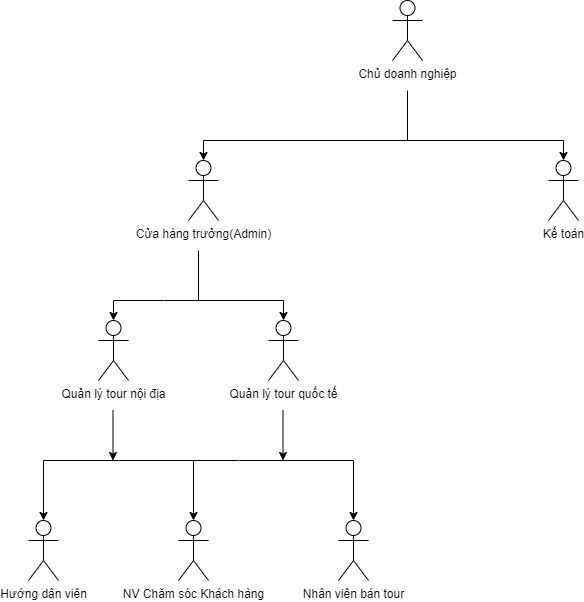
\includegraphics[width = 0.65\linewidth]{figures/Untitled Diagram.drawio (6).png}).png}
    \caption{Sơ đồ tổ chức cấp quản lý của  HAPPY TOUR.}
    \label{fig:example_1}
\end{figure}

\textTo{
\begin{itemize}
\item Khách hàng sử dụng tài khoản đăng nhập vào trang web (được phép tự đăng ký nếu chưa có) xem danh sách các tour, xem chi tiết một tour. Sau đó tiến thành đặt vé tour (nếu hài lòng) và thanh toán bằng thẻ ngân hàng hoặc thanh toán trực tiếp. 
\item Chat với bộ phận chăm sóc khách hàng nếu cần tư vấn và giải đáp thắc mắc.
\item Quản lý cập nhận thông tin cá nhân.
\end{itemize}

}

\begin{figure}[ht]
    \centering
    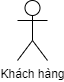
\includegraphics[width = 0.1\linewidth]{figures/Khách Hàng.png}
    \caption{Khách Hàng HAPPY TOUR.}
    \label{fig:example_1}
\end{figure}

\subsubsection{Các nhóm chức năng của hệ thống}

\begin{itemize}
\item Nhóm chức năng xem thông tin: Bao gồm xem tất cả thông tin khách hàng cho  phép, xem thông tin tour du lịch, chương trình khuyến mãi, ..., thông báo.
\item Nhóm chức năng quản lý: Quản lý nhân viên, quản lý thông tin tour du lịch, quản lý danh sách khách hàng tham gia tour, quản lý khuyến mãi, quản lý thông tin cá nhân khách hàng,...,quản lý tiền.
\item Nhóm chức năng tiếp nhận và xử lý: Kết nối liên lạc giữa khách hàng với các cấp quan lý, xử lý yêu cầu.
\end{itemize}

\subsubsection{Xác định các chức năng chính của hệ thống}

Tất cả các User phải đăng nhập mới được cấp quyền thực hiện các chức năng trong hệ thống ( ngoài trừ chức năng đăng ký của Khách Hàng)

\begin{figure}[ht]
    \centering
    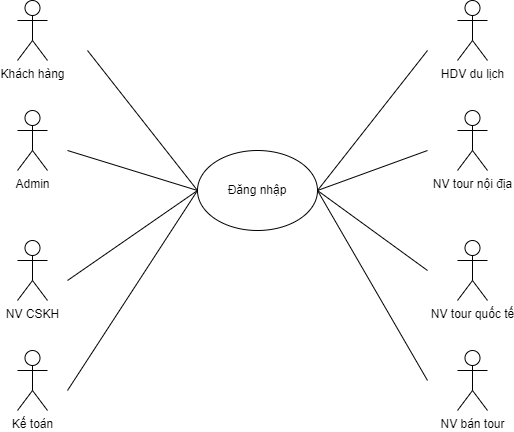
\includegraphics[width = 1.15\linewidth]{figures/Sub-UseCase-Đăng nhập.png}
    \caption{Chức năng đăng nhập.}
    \label{fig:example_1}
\end{figure}

\vspace{10cm}

\begin{enumerate}
\item Khách hàng


\begin{itemize}
\item Tạo tài khoản người dùng và đăng nhập vào Website và quản lí thông tin cá nhân.
\item Xem trang danh sách tour tổng quan, xem chi tiết tour, thanh toán qua ứng dụng thứ 3, theo dỗi hành trình di chuyển bằng app nội bộ được cung cấp khi đi tour.
\item Xem lại các tour đã đặt và đánh giá tour, hủy tour ( phải chờ phản hồi từ công ty)
\item Nhận thông báo về tour cũng như hóa đơn qua mail, nhận thông tin khuyến mãi.
\item Chat trực tuyến với bộ phận CSKH trên website
\end{itemize}

\begin{figure}[ht]
    \centering
    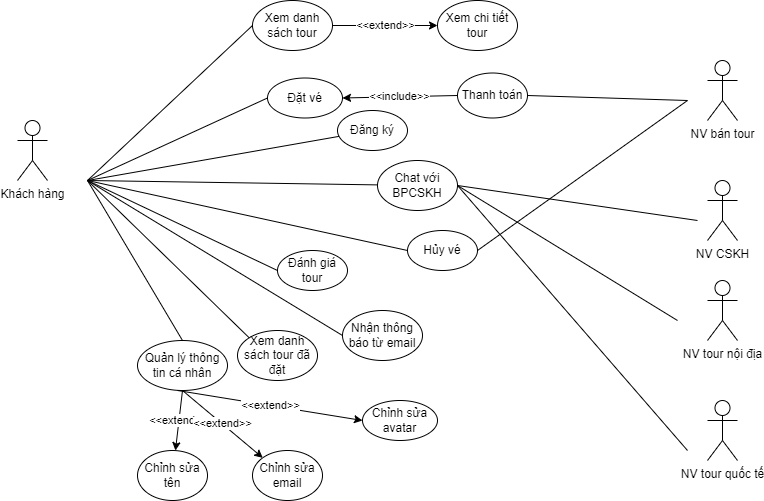
\includegraphics[width = 1.15\linewidth]{figures/Sub-UseCase-KhachHang.png}
    \caption{Chức năng của Khách Hàng.}
    \label{fig:example_1}
\end{figure}

\vspace{5cm}

\item Nhân viên phụ trách thông tin tour nội địa

\begin{itemize}
\item Được cung cấp tài khoản trang nội bộ để quản lí cập nhật (thêm, xóa, chỉnh sửa) thông tin tour du lịch nội địa ( bao gồm cả thông tin khách sạn và phương tiện di chuyển)
\item Được sử dụng chức năng trò chuyện trực tuyến trên website để hỗ trợ bộ phận CSKH.
\end{itemize}

\begin{figure}[ht]
    \centering
    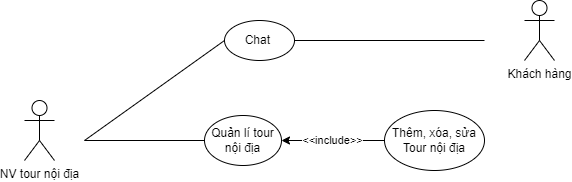
\includegraphics[width = 0.98\linewidth]{figures/Sub-UseCase-TourNoiDia.png}
    \caption{Sub UseCase Tour NoiDia.}
    \label{fig:example_1}
\end{figure}

\vspace{1cm}

\item Nhân viên phụ trách thông tin tour quốc tế

\begin{itemize}
\item Chức năng tương tự với nhân viên tour nội địa nhưng bổ sung thêm thông tin tiêm chủng và visa.
\end{itemize}

\begin{figure}[ht]
    \centering
    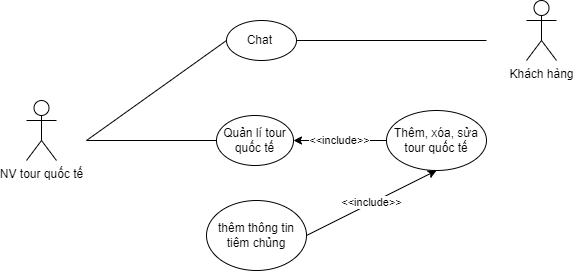
\includegraphics[width = 0.93\linewidth]{figures/Sub-UseCase-TourQuocTe.png}
    \caption{Sub UseCase Tour QuocTe.}
    \label{fig:example_1}
\end{figure}

\vspace{10cm}

\item Hướng dẫn viên du lịch (thuộc sở hữu của công ty)

\begin{itemize}
\item Xem những tour đã được phân công
\item Xem chi tiết thông tin tour bao gồm lịch trình, hành khách, phương tiện di chuyển, khách sạn.
\end{itemize}

\begin{figure}[ht]
    \centering
    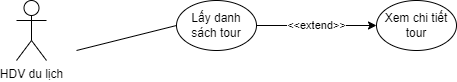
\includegraphics[width = 0.7\linewidth]{figures/Sub-UseCase-HDVdulich.png}
    \caption{Sub UseCase HDVdulich.}
    \label{fig:example_1}
\end{figure}

\item Nhân viên chăm sóc khách hàng

\begin{itemize}
\item Tư vấn và giải đáp các yêu cầu mà khách hàng gửi tin nhắn qua website.
\end{itemize}

\begin{figure}[ht]
    \centering
    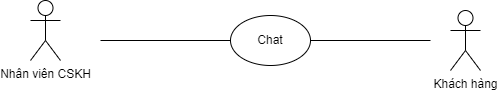
\includegraphics[width = 0.7\linewidth]{figures/Sub-UseCase-CSKH.png}
    \caption{Sub UseCase CSKH.}
    \label{fig:example_1}
\end{figure}

\item Kế toán

\begin{itemize}
\item Thống kê dữ liệu về tour và khách hàng và tài chính theo tuần, tháng, năm
\item Xuất báo cáo theo tuần, tháng, năm
\item Tính lương dựa theo số liệu điểm danh của phần mềm thứ 3 tích hợp dữ liệu sẳn vào hệ thống
\end{itemize}

\begin{figure}[ht]
    \centering
    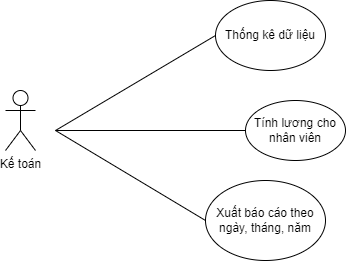
\includegraphics[width = 0.3\linewidth]{figures/Sub-UseCase-KeToan.png}
    \caption{Sub UseCase KeToan.}
    \label{fig:example_1}
\end{figure}

\item Nhiên viên bán tour

\begin{itemize}
\item Được cấp tài khoản nội bộ để xem danh sách tour và xử lý yêu cầu thanh toán, đồng thời phản hồi nếu có sự việc xảy ra.
\end{itemize}

\begin{figure}[ht]
    \centering
    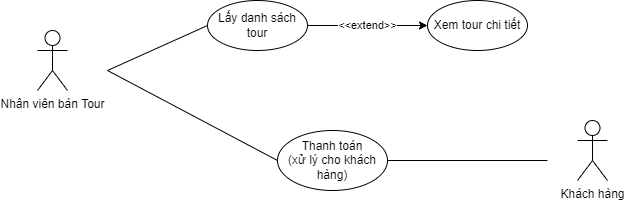
\includegraphics[width = 0.7\linewidth]{figures/Sub-UseCase-NVbanTour.png}
    \caption{Sub UseCase NVbanTour.}
    \label{fig:example_1}
\end{figure}

\vspace{5cm}

\item Cửa hàng trưởng - Admin

\begin{itemize}
\item Thực hiện được tất cả các chức năng của các nhân viên khác có toàn quyền trong hệ thống. 
\item Có thể phân bổ quyền hạn nhân viên.
\end{itemize}

\end{enumerate}

\begin{figure}[ht]
    \centering
    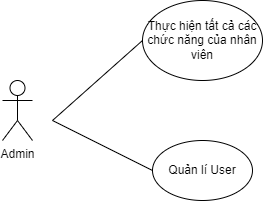
\includegraphics[width = 0.4\linewidth]{figures/Sub-UseCase-Admin.png}
    \caption{Sub-UseCase-Admin.}
    \label{fig:example_1}
\end{figure}

\vspace{10cm}

\begin{figure}[ht]
    \centering
    \includegraphics[width = 1.2\linewidth]{figures/Use Case.png}
    \caption{Sub-UseCase.}
    \label{fig:example_1}
\end{figure}

\vspace{10cm}





\vspace{10cm}

\subsubsection{Use case description}

\addcontentsline{lot}{table}{USE-CASE DESCRIPTION}

\begin{center}
    \begin{tabular}{|ll|}
    \hline
    \multicolumn{2}{|l|}{\centerline{\textbf{Quản lý xác thực người dùng.}}} \\[0.5cm] \hline
    \multicolumn{1}{|l|}{\textbf{Use Case ID}} & \begin{tabular}{p{10cm}} UC-1\end{tabular}  \\[0.3cm] \hline 
    \multicolumn{1}{|l|}{\textbf{Description}} &  \begin{tabular}{p{12cm}} Là người dùng, tôi muốn đăng nhập vào ứng dụng để sử dụng dịch vụ từ ứng dụng.
    \end{tabular}\\[0.5cm] \hline
    \multicolumn{1}{|l|}{\textbf{Actor}} & \begin{tabular}{p{12cm}} Khách hàng, Quản lý, Kế t Admin\end{tabular}  \\[0.3cm] \hline 
    
    
    \multicolumn{1}{|l|}{\textbf{Pre-Condition(s):	
}} & \begin{tabular}{p{12cm}} 
\begin{itemize}
\item Tài khoản người dùng đã được tạo sẵn
\item Tài khoản người dùng đã được phân quyền
\item Thiết bị của người dùng đã được kết nối internet khi thực hiện đăng nhập
\end{itemize}
\end{tabular} \\[0.5cm] \hline

    \multicolumn{1}{|l|}{\textbf{Trigger}} & \begin{tabular}{p{12cm}} Người dùng yêu cầu đăng nhập vào ứng dụng Happy-Tour\end{tabular} \\[0.5cm] \hline

    \multicolumn{1}{|l|}{\textbf{Post-Condition(s):	
}} & \begin{tabular}{p{12cm}} 
\begin{itemize}
\item Người dùng đăng nhập ứng dụng thành công
\item Hệ thống ghi nhận hoạt động đăng nhập thành công
\end{itemize}
.\end{tabular} \\[0.5cm] \hline
    \multicolumn{1}{|l|}{\textbf{Basic Flow	}} &  \begin{tabular}{p{12cm}} 
        \begin{enumerate}
        \item Người dung truy cập vào website.
        \item Người dùng chọn nút login
        \item Người dùng nhập tài khoản và chọn đăng nhập
        \end{enumerate}
    \end{tabular}\\[0.5cm] \hline
 
    \multicolumn{1}{|l|}{\textbf{Exception Flow	}} & \begin{tabular}{p{12cm}} 
    
    \begin{itemize}
    \item Hệ thống xác thực thông tin đăng nhập không thành.
    \item     Người dùng chọn lệnh lấy lại mật khẩu
    \end{itemize}

    \end{tabular} \\[0.5cm] \hline
    
    \hline 
    \multicolumn{1}{|l|}{\textbf{Non-Functional}} & \begin{tabular}{p{12cm}} 
    Mật khẩu của người dùng phải được hash bằng bcrypt
    \end{tabular}  \\[0.5cm] \hline
    
    \end{tabular}
    \captionof{table}{Đăng nhập xác thực người dùng}\label{tbl:nicetablelesstable}
\end{center}
% ____





% Test
\begin{center}
    \begin{tabular}{|ll|}
    \hline
    \multicolumn{2}{|l|}{\centerline{\textbf{Xem danh sách tour.}}} \\[0.5cm] \hline
    \multicolumn{1}{|l|}{\textbf{Use Case ID}} & \begin{tabular}{p{10cm}} UC-2\end{tabular}  \\[0.3cm] \hline 
    \multicolumn{1}{|l|}{\textbf{Description}} &  \begin{tabular}{p{12cm}} Là người dùng, tôi muốn vào ứng dụng để xem danh sách các tour của Happy-Tour.
    \end{tabular}\\[0.5cm] \hline
    \multicolumn{1}{|l|}{\textbf{Actor}} & \begin{tabular}{p{12cm}} Khách hàng\end{tabular}  \\[0.3cm] \hline 
    
    \multicolumn{1}{|l|}{\textbf{Pre-Condition(s):	
}} & \begin{tabular}{p{12cm}} 
    \begin{itemize}
    \item Thiết bị của người dùng đã được kết nối internet khi thực hiện đăng nhập
    \item Người dùng truy cập website
    \end{itemize}
    \end{tabular} \\[0.5cm] \hline

    \multicolumn{1}{|l|}{\textbf{Trigger}} & \begin{tabular}{p{12cm}} \end{tabular} \\[0.5cm] \hline
    
    \multicolumn{1}{|l|}{\textbf{Post-Condition(s):	
}} & \begin{tabular}{p{12cm}} 
    Người dùng xem được danh sách tour.
    .\end{tabular} \\[0.5cm] \hline
    
    \multicolumn{1}{|l|}{\textbf{Basic Flow	}} &  \begin{tabular}{p{12cm}} 
        \begin{enumerate}
        \item Người dùng truy cập vào website.
        \item Người dùng duyệt danh sách tour có trên trang.\end{enumerate}
    \end{tabular}\\[0.5cm] \hline
 
    \multicolumn{1}{|l|}{\textbf{Exception Flow	}} & \begin{tabular}{p{12cm}} 
    
    \begin{itemize}
    \item Hiện không có tour nào trên hệ thống.
    \item Người quản lý đang cập nhật lại danh sách tour.
    \end{itemize}

    \end{tabular} \\[0.5cm] \hline
    
    \multicolumn{1}{|l|}{\textbf{Non-Functional}} & \begin{tabular}{p{12cm}} 
   
    \begin{itemize}
    \item  Các tour được nhiều người chọn và đem lại doanh thu sẽ ở trên cùng.
    % \item     Các tour đem lại nhiều lợi nhuận hơn phải làm nổi bật bắt mắt.
    \end{itemize}

    \end{tabular}  \\[0.5cm] \hline
    
    \end{tabular}
    \captionof{table}{Xem danh sách tour}\label{tbl:nicetablelesstable}
\end{center}
% ----

\begin{center}
    \begin{tabular}{|ll|}
    \hline
    \multicolumn{2}{|l|}{\centerline{\textbf{Đặt vé.}}} \\[0.5cm] \hline
    \multicolumn{1}{|l|}{\textbf{Use Case ID}} & \begin{tabular}{p{10cm}} UC-3\end{tabular}  \\[0.3cm] \hline 
    \multicolumn{1}{|l|}{\textbf{Description}} &  \begin{tabular}{p{12cm}} Người dùng muốn đặt chổ tham gia tour du lịch.
    \end{tabular}\\[0.5cm] \hline
    \multicolumn{1}{|l|}{\textbf{Actor}} & \begin{tabular}{p{12cm}} Khách hàng, Nhân viên bán tour.\end{tabular}  \\[0.3cm] \hline 
    \multicolumn{1}{|l|}{\textbf{Pre-Condition(s):	
}} & \begin{tabular}{p{12cm}} 

    \begin{itemize}
    \item Tài khoản người dùng đã được tạo sẵn
    \end{itemize}
    \end{tabular} \\[0.5cm] \hline

    \multicolumn{1}{|l|}{\textbf{Trigger}} & \begin{tabular}{p{12cm}} Khách hàng nhấn vào nút đặt vé tour du lịch.\end{tabular} \\[0.5cm] \hline
    
    \multicolumn{1}{|l|}{\textbf{Post-Condition(s):	
}} & \begin{tabular}{p{12cm}} 
    \begin{itemize}
    \item Người dùng được thông báo đã đặt vé thành công trên website
    \item Hệ thống ghi nhận hoạt động
    \item Khách hàng nhận được mail thông báo chi tiết
    \end{itemize}
    .\end{tabular} \\[0.5cm] \hline
    
    \multicolumn{1}{|l|}{\textbf{Basic Flow	}} &  \begin{tabular}{p{12cm}} 
        \begin{enumerate}
        \item Người dụng chọn tour du lịch mình mong muốn trên web 
        \item Người dùng vào giỏ hàng trên cùng bên phải
        \item Người dùng nhập thông tin thẻ tín dụng và chọn "Thanh Toán"
        \item Người dùng xác nhận lại thông tin trên màn hình và kiểm tra mail gửi tới
        \end{enumerate}
    \end{tabular}\\[0.5cm] \hline
 
    \multicolumn{1}{|l|}{\textbf{Exception Flow	}} & \begin{tabular}{p{12cm}} 
    
    \begin{itemize}
    \item Lỗi từ hệ thống
    \item Thông tin thẻ tín dụng sai
    \end{itemize}
    \end{tabular} \\[0.5cm] \hline
    
    \multicolumn{1}{|l|}{\textbf{Non-Functional}} & \begin{tabular}{p{12cm}} 
    Hỗ trợ nhiều loại thẻ tín dụng.
    \end{tabular}  \\[0.5cm] \hline
    
    \end{tabular}
    \captionof{table}{Đặt vé}\label{tbl:nicetablelesstable}
\end{center}
% ---

\begin{center}
    \begin{tabular}{|ll|}
    \hline
    \multicolumn{2}{|l|}{\centerline{\textbf{Hủy vé.}}} \\[0.5cm] \hline
    \multicolumn{1}{|l|}{\textbf{Use Case ID}} & \begin{tabular}{p{10cm}} UC-4\end{tabular}  \\[0.3cm] \hline 
    \multicolumn{1}{|l|}{\textbf{Description}} &  \begin{tabular}{p{12cm}} Người dùng muốn hủy đặt chổ tham gia tour du lịch.
    \end{tabular}\\[0.5cm] \hline
    \multicolumn{1}{|l|}{\textbf{Actor}} & \begin{tabular}{p{12cm}} Khách hàng, Nhân viên bán tour.\end{tabular}  \\[0.3cm] \hline 
    \multicolumn{1}{|l|}{\textbf{Pre-Condition(s):	
}} & \begin{tabular}{p{12cm}} 

    \begin{itemize}
    \item Tài khoản người dùng đã được tạo sẵn
    \item Tài khoản người dùng đã được phân quyền
    \item Tour du lịch ở trạng thái đã thanh toán chưa tiến hành.
    \end{itemize}
    \end{tabular} \\[0.5cm] \hline

    \multicolumn{1}{|l|}{\textbf{Trigger}} & \begin{tabular}{p{12cm}} Khách hàng nhấn vào nút hủy đặt vé tour du lịch trong danh sách tour đã đặt.\end{tabular} \\[0.5cm] \hline
    
    \multicolumn{1}{|l|}{\textbf{Post-Condition(s):	
}} & \begin{tabular}{p{12cm}} 
    \begin{itemize}
    \item Người dùng được thông báo hủy vé thành công trên website
    \item Hệ thống ghi nhận hoạt động
    \item Khách hàng nhận được mail thông báo chi tiết
    \end{itemize}
    .\end{tabular} \\[0.5cm] \hline
    
    \multicolumn{1}{|l|}{\textbf{Basic Flow	}} &  \begin{tabular}{p{12cm}} 
        \begin{enumerate}
        \item Người dùng vào profile cá nhân 
        \item Người dùng vào mục " MyBooking" bên trái
        \item Người dùng chọn tour muốn hủy
        \item Người dùng chọn "Accept"
        \end{enumerate}
    \end{tabular}\\[0.5cm] \hline
 
    \multicolumn{1}{|l|}{\textbf{Exception Flow	}} & \begin{tabular}{p{12cm}} 
    
    \begin{itemize}
    \item Còn 2 tuần tour bắt đầu
    \item Tour đã bị hủy trước đó
    \end{itemize}
    \end{tabular} \\[0.5cm] \hline
    
    \multicolumn{1}{|l|}{\textbf{Non-Functional}} & \begin{tabular}{p{12cm}} 
    % Cho phép khách hàng chuyển tiền thanh toán sang tour khách.
    \end{tabular}  \\[0.5cm] \hline
    
    \end{tabular}
    \captionof{table}{Hủy vé}\label{tbl:nicetablelesstable}
\end{center}

% ---
\begin{center}
    \begin{tabular}{|ll|}
    \hline
    \multicolumn{2}{|l|}{\centerline{\textbf{Quản lí thông tin cá nhân.}}} \\[0.5cm] \hline
    \multicolumn{1}{|l|}{\textbf{Use Case ID}} & \begin{tabular}{p{10cm}} UC-5\end{tabular}  \\[0.3cm] \hline 
    \multicolumn{1}{|l|}{\textbf{Description}} &  \begin{tabular}{p{12cm}} Khách hàng có nhu cầu cập nhật thông tin cá nhân
    \end{tabular}\\[0.5cm] \hline
    \multicolumn{1}{|l|}{\textbf{Actor}} & \begin{tabular}{p{12cm}} Khách hàng, Các quản lí, Admin.\end{tabular}  \\[0.3cm] \hline 
    \multicolumn{1}{|l|}{\textbf{Pre-Condition(s):	
}} & \begin{tabular}{p{12cm}} 

    \begin{itemize}
    \item Tài khoản người dùng đã được tạo sẵn
    \item Tài khoản người dùng đã được phân quyền
    \item Thông tin đã được tải lên
    \end{itemize}
    \end{tabular} \\[0.5cm] \hline

    \multicolumn{1}{|l|}{\textbf{Trigger}} & \begin{tabular}{p{12cm}} Người dùng chọn vào tên mình trên cùng trang web .\end{tabular} \\[0.5cm] \hline
    
    \multicolumn{1}{|l|}{\textbf{Post-Condition(s):	
}} & \begin{tabular}{p{12cm}} 
    \begin{itemize}
    \item Người dùng truy cập được thông tin cá nhân
    \item Hệ thống ghi nhận sửa đổi (nếu có)
    \item Người dùng nhận được mail thông báo cập nhật.
    \end{itemize}
    .\end{tabular} \\[0.5cm] \hline
    
    \multicolumn{1}{|l|}{\textbf{Basic Flow	}} &  \begin{tabular}{p{12cm}} 
        \begin{enumerate}
        \item Người dùng đăng nhập vào hệ thống 
        \item Người dùng nhấn vào tên và avatar trên cùng trang web
        \item Người dùng xem thông tin
        \item Người dùng cập nhật thông tin(nếu có):Tên, mật khẩu , Ảnh đại diện, địa chỉ, thông tin thẻ,...
        \end{enumerate}
    \end{tabular}\\[0.5cm] \hline
 
    \multicolumn{1}{|l|}{\textbf{Exception Flow	}} & \begin{tabular}{p{12cm}} 
    
    \begin{itemize}
    \item Đăng nhập không thành công
    \item Không có quyền truy cập
    \end{itemize}
    \end{tabular} \\[0.5cm] \hline
    
    \multicolumn{1}{|l|}{\textbf{Non-Functional}} & \begin{tabular}{p{12cm}} 
    Tất cả thông tin phải được bảo mật.
    \end{tabular}  \\[0.5cm] \hline
    
    \end{tabular}
    \captionof{table}{Quản lí thông tin}\label{tbl:nicetablelesstable}
\end{center}
% ---

\begin{center}
    \begin{tabular}{|ll|}
    \hline
    \multicolumn{2}{|l|}{\centerline{\textbf{Xem danh sách tour đã đặt.}}} \\[0.5cm] \hline
    \multicolumn{1}{|l|}{\textbf{Use Case ID}} & \begin{tabular}{p{10cm}} UC-6\end{tabular}  \\[0.3cm] \hline 
    \multicolumn{1}{|l|}{\textbf{Description}} &  \begin{tabular}{p{12cm}} Người dùng duyệt xem danh sách tour đã đặt.
    \end{tabular}\\[0.5cm] \hline
    \multicolumn{1}{|l|}{\textbf{Actor}} & \begin{tabular}{p{12cm}} Khách hàng\end{tabular}  \\[0.3cm] \hline 
    \multicolumn{1}{|l|}{\textbf{Pre-Condition(s):	
}} & \begin{tabular}{p{12cm}} 

    \begin{itemize}
    \item Tài khoản người dùng đã được phân quyền
    \item Khách hàng đã đặt tour trước đó
    \end{itemize}
    \end{tabular} \\[0.5cm] \hline

    \multicolumn{1}{|l|}{\textbf{Trigger}} & \begin{tabular}{p{12cm}} Người dùng nhấn vào "MyBooking" trong profile.\end{tabular} \\[0.5cm] \hline
    
    \multicolumn{1}{|l|}{\textbf{Post-Condition(s):	
}} & \begin{tabular}{p{12cm}} 
    Hiển thị các tour Khách hàng đã thanh toán
    .\end{tabular} \\[0.5cm] \hline
    
    \multicolumn{1}{|l|}{\textbf{Basic Flow	}} &  \begin{tabular}{p{12cm}} 
        \textbf{Khách hàng}
        \begin{itemize}
        \item Khách hàng truy cập được thông tin cá nhân
        \item Khách hàng chọn "MyBooking"
        \end{itemize}
        % \textbf{Nhân viên chăm sóc, Nhân viên bán vé, Admin}
        % \begin{itemize}
        % \item NV truy cập vào thông tin khách hàng
        % \item Chọn "My tour"
        % \end{itemize}
    \end{tabular}\\[0.5cm] \hline
 
    \multicolumn{1}{|l|}{\textbf{Exception Flow	}} & \begin{tabular}{p{12cm}} 
    
    \begin{itemize}
    \item Khách hàng không có tour đã đặt
    \end{itemize}
    \end{tabular} \\[0.5cm] \hline
    
    \multicolumn{1}{|l|}{\textbf{Non-Functional}} & \begin{tabular}{p{12cm}} 
    % Chương trình khuyến mãi dựa trên sở thich đặt tour trước đó của khách hàng.
    \end{tabular}  \\[0.5cm] \hline
    
    \end{tabular}
    \captionof{table}{Xem danh sách tour đã đặt}\label{tbl:nicetablelesstable}
\end{center}

% ---

\begin{center}
    \begin{tabular}{|ll|}
    \hline
    \multicolumn{2}{|l|}{\centerline{\textbf{Lấy danh sách khách hàng tham gia tour}}} \\[0.5cm] \hline
    \multicolumn{1}{|l|}{\textbf{Use Case ID}} & \begin{tabular}{p{10cm}} UC-7\end{tabular}  \\[0.3cm] \hline 
    \multicolumn{1}{|l|}{\textbf{Description}} &  \begin{tabular}{p{12cm}} Các cấp quản lí lấy danh sách khách hàng tham gia tour.
    \end{tabular}\\[0.5cm] \hline
    \multicolumn{1}{|l|}{\textbf{Actor}} & \begin{tabular}{p{12cm}} Hướng dẫn viên, Nhân viên bán tour, Admin.\end{tabular}  \\[0.3cm] \hline 
    \multicolumn{1}{|l|}{\textbf{Pre-Condition(s):	
}} & \begin{tabular}{p{12cm}} 

    \begin{itemize}
    \item Tài khoản người dùng đã được phân quyền
    \item Có hành khách tham gia tour
    \end{itemize}
    \end{tabular} \\[0.5cm] \hline

    \multicolumn{1}{|l|}{\textbf{Trigger}} & \begin{tabular}{p{12cm}} Người dùng muốn xem thông tin khách đã đặt tour.\end{tabular} \\[0.5cm] \hline
    
    \multicolumn{1}{|l|}{\textbf{Post-Condition(s):	
}} & \begin{tabular}{p{12cm}} 
    Hiển thị các khách hàng đã đặt tour
    .\end{tabular} \\[0.5cm] \hline
    
    \multicolumn{1}{|l|}{\textbf{Basic Flow	}} &  \begin{tabular}{p{12cm}} 
        \begin{itemize}
        \item Người dùng đăng nhập vào hệ thống nội bộ
        \item Người dùng chọn "tour list (available)"\end{itemize}
    \end{tabular}\\[0.5cm] \hline
 
    \multicolumn{1}{|l|}{\textbf{Exception Flow	}} & \begin{tabular}{p{12cm}} 
    
    \begin{itemize}
    \item Không có quyền truy cập
    \end{itemize}
    \end{tabular} \\[0.5cm] \hline
    
    \multicolumn{1}{|l|}{\textbf{Non-Functional}} & \begin{tabular}{p{12cm}} 
    % Xác nhận tham gia chuyến đi
    \end{tabular}  \\[0.5cm] \hline
    
    \end{tabular}
    \captionof{table}{Lấy danh sách khách hàng tham gia tour}\label{tbl:nicetablelesstable}
\end{center}
% ---

% \begin{center}
%     \begin{tabular}{|ll|}
%     \hline
%     \multicolumn{2}{|l|}{\centerline{\textbf{Kiêm tra tình trạng tour}}} \\[0.5cm] \hline
%     \multicolumn{1}{|l|}{\textbf{Use Case ID}} & \begin{tabular}{p{10cm}} UC-8\end{tabular}  \\[0.3cm] \hline 
%     \multicolumn{1}{|l|}{\textbf{Description}} &  \begin{tabular}{p{12cm}} Các cấp quản lí muốn kiểm tra tình trạng khách hàng tham gia tour.
%     \end{tabular}\\[0.5cm] \hline
%     \multicolumn{1}{|l|}{\textbf{Actor}} & \begin{tabular}{p{12cm}} Quản lí tour nội địa(quốc tế), nhân viên chăm sóc khách hàng, Admin.\end{tabular}  \\[0.3cm] \hline 
%     \multicolumn{1}{|l|}{\textbf{Pre-Condition(s):	
% }} & \begin{tabular}{p{12cm}} 

%     \begin{itemize}
%     \item Tài khoản người dùng đã được phân quyền
%     \item Có hành khách tham gia tour
%     \end{itemize}
%     \end{tabular} \\[0.5cm] \hline

%     \multicolumn{1}{|l|}{\textbf{Trigger}} & \begin{tabular}{p{12cm}} Kiểm tra lần cuối trước khi tiến hành tour du lịch.\end{tabular} \\[0.5cm] \hline
    
%     \multicolumn{1}{|l|}{\textbf{Post-Condition(s):	
% }} & \begin{tabular}{p{12cm}} 
%     Hiển thị thông tin khách hàng đã đặt tour: Tình trạng xác nhận tham gia, visa, tình trạng tiêm chuẩn, tình trạng sức khỏe, thanh toán,.. của khách hàng.
%     .\end{tabular} \\[0.5cm] \hline
    
%     \multicolumn{1}{|l|}{\textbf{Basic Flow	}} &  \begin{tabular}{p{12cm}} 
%         \begin{itemize}
%         \item Người dùng vào "profile"
%         \item Người dùng chọn "All tour"
%         \item Người dùng chọn thẻ tour muốn kiểm tra
%         \end{itemize}
%     \end{tabular}\\[0.5cm] \hline
 
%     \multicolumn{1}{|l|}{\textbf{Exception Flow	}} & \begin{tabular}{p{12cm}} 
    
%     \begin{itemize}
%     \item Không có quyền truy cập
%     \item Không có khách hàng tham gia tour
%     \item Tour đã được tiến hành
%     \end{itemize}
%     \end{tabular} \\[0.5cm] \hline
    
%     \multicolumn{1}{|l|}{\textbf{Non-Functional}} & \begin{tabular}{p{12cm}} 
%     Thay vị trí trống nếu có khách hàng cancel.
%     \end{tabular}  \\[0.5cm] \hline
    
%     \end{tabular}
%     \captionof{table}{Kiêm tra tình trạng tour}\label{tbl:nicetablelesstable}
% \end{center}

% ---
\begin{center}
    \begin{tabular}{|ll|}
    \hline
    \multicolumn{2}{|l|}{\centerline{\textbf{Kết nối nhân viên chắm sóc khách hàng với khách}}} \\[0.5cm] \hline
    \multicolumn{1}{|l|}{\textbf{Use Case ID}} & \begin{tabular}{p{10cm}} UC-9\end{tabular}  \\[0.3cm] \hline 
    \multicolumn{1}{|l|}{\textbf{Description}} &  \begin{tabular}{p{12cm}} Khách hàng cần tư vấn hỏi đáp bằng cách chat với nhân viên chăm sóc qua website.
    \end{tabular}\\[0.5cm] \hline
    \multicolumn{1}{|l|}{\textbf{Actor}} & \begin{tabular}{p{12cm}} Khách hàng, Nhân viên chắm sóc khách hàng.\end{tabular}  \\[0.3cm] \hline 
    \multicolumn{1}{|l|}{\textbf{Pre-Condition(s):	
}} & \begin{tabular}{p{12cm}} 

    \begin{itemize}
    \item Tài khoản người dùng đã được phân quyền
    \item Có khách hàng liên hệ
    \end{itemize}
    \end{tabular} \\[0.5cm] \hline

    \multicolumn{1}{|l|}{\textbf{Trigger}} & \begin{tabular}{p{12cm}} Khách hàng muốn liên lạc với nhân viên chắm sóc khách hàng.\end{tabular} \\[0.5cm] \hline
    
    \multicolumn{1}{|l|}{\textbf{Post-Condition(s):	
}} & \begin{tabular}{p{12cm}} 
    khách hàng và nhân viên chăm sóc kết nối thành công với nhau .
    .\end{tabular} \\[0.5cm] \hline
    
    \multicolumn{1}{|l|}{\textbf{Basic Flow	}} &  \begin{tabular}{p{12cm}} 
        \textbf{Khách hàng}
        \begin{itemize}
        \item Khách hàng vào website
        \item Khách hàng chọn vào biểu tượng CSKH
        \item Khách hàng nhập tin nhắn trong ô chat và gửi đi
        \end{itemize}
        \textbf{Nhân viên chăm sóc khách hàng}
        \begin{itemize}
        \item Nhân viên vào website
        \item Nhân viên nhận được thông báo
        \item Kiểm tra tin nhắn hiển thị và trả lời khách hàng
        \end{itemize}
    \end{tabular}\\[0.5cm] \hline
 
    \multicolumn{1}{|l|}{\textbf{Exception Flow	}} & \begin{tabular}{p{12cm}} 
    Không có Nhân viên CSKH nào
    \end{tabular} \\[0.5cm] \hline
    
    \multicolumn{1}{|l|}{\textbf{Non-Functional}} & \begin{tabular}{p{12cm}} 
    Thời gian hồi đáp nhanh
    \end{tabular}  \\[0.5cm] \hline
    
    \end{tabular}
    \captionof{table}{Kết nối nhân viên chắm sóc khách hàng với khách}\label{tbl:nicetablelesstable}
\end{center}

% ---

\begin{center}
    \begin{tabular}{|ll|}
    \hline
    \multicolumn{2}{|l|}{\centerline{\textbf{Tour nội địa}}} \\[0.5cm] \hline
    \multicolumn{1}{|l|}{\textbf{Use Case ID}} & \begin{tabular}{p{10cm}} UC-10\end{tabular}  \\[0.3cm] \hline 
    \multicolumn{1}{|l|}{\textbf{Description}} &  \begin{tabular}{p{12cm}} Quản lý cập nhật tour nội địa.
    \end{tabular}\\[0.5cm] \hline
    \multicolumn{1}{|l|}{\textbf{Actor}} & \begin{tabular}{p{12cm}} Quản lý tour nội địa, Admin.\end{tabular}  \\[0.3cm] \hline 
    \multicolumn{1}{|l|}{\textbf{Pre-Condition(s):	
}} & \begin{tabular}{p{12cm}} 

    Tài khoản người dùng đã được phân quyền
    \end{tabular} \\[0.5cm] \hline

    \multicolumn{1}{|l|}{\textbf{Trigger}} & \begin{tabular}{p{12cm}} Quản lý chọn cập nhật tour du lịch nội địa.\end{tabular} \\[0.5cm] \hline
    
    \multicolumn{1}{|l|}{\textbf{Post-Condition(s):	
}} & \begin{tabular}{p{12cm}} 
    Tour du lịch nội địa được cập nhật thành công trên hệ thống.
    .\end{tabular} \\[0.5cm] \hline
    
    \multicolumn{1}{|l|}{\textbf{Basic Flow	}} &  \begin{tabular}{p{12cm}} 
        \begin{itemize}
        \item Quản lý đăng nhập vào website hệ thống
        \item Quản lý vào "Domestic tour" để truy cập danh sách.
        \item Quản lý thêm xóa sửa tour nội địa
        \end{itemize}
    \end{tabular}\\[0.5cm] \hline
 
    \multicolumn{1}{|l|}{\textbf{Exception Flow	}} & \begin{tabular}{p{12cm}} 
    Nhân viên không phải quản lí của tour
    \end{tabular} \\[0.5cm] \hline
    
    \multicolumn{1}{|l|}{\textbf{Non-Functional}} & \begin{tabular}{p{12cm}} 
    Tour du lịch được cập nhật thường xuyên
    \end{tabular}  \\[0.5cm] \hline
    
    \end{tabular}
    \captionof{table}{Tour nội địa}\label{tbl:nicetablelesstable}
\end{center}

% ---

\begin{center}
    \begin{tabular}{|ll|}
    \hline
    \multicolumn{2}{|l|}{\centerline{\textbf{Tour quốc tế}}} \\[0.5cm] \hline
    \multicolumn{1}{|l|}{\textbf{Use Case ID}} & \begin{tabular}{p{10cm}} UC-11\end{tabular}  \\[0.3cm] \hline 
    \multicolumn{1}{|l|}{\textbf{Description}} &  \begin{tabular}{p{12cm}} Quản lý cập nhật tour quốc tế.
    \end{tabular}\\[0.5cm] \hline
    \multicolumn{1}{|l|}{\textbf{Actor}} & \begin{tabular}{p{12cm}} Quản lý tour quốc tế, Admin.\end{tabular}  \\[0.3cm] \hline 
    \multicolumn{1}{|l|}{\textbf{Pre-Condition(s):	
}} & \begin{tabular}{p{12cm}} 

    Tài khoản người dùng đã được phân quyền
    \end{tabular} \\[0.5cm] \hline

    \multicolumn{1}{|l|}{\textbf{Trigger}} & \begin{tabular}{p{12cm}} Quản lý chọn cập nhật tour du lịch quốc tế.\end{tabular} \\[0.5cm] \hline
    
    \multicolumn{1}{|l|}{\textbf{Post-Condition(s):	
}} & \begin{tabular}{p{12cm}} 
    Tour du lịch nội địa được cập nhật thành công trên hệ thống.
    .\end{tabular} \\[0.5cm] \hline
    
    \multicolumn{1}{|l|}{\textbf{Basic Flow	}} &  \begin{tabular}{p{12cm}} 
        \begin{itemize}
        \item Quản lý đăng nhập vào website hệ thống
        \item Quản lý vào "International tour" để truy cập danh sách.
        \item Quản lý thêm xóa sửa tour nội địa
        \end{itemize}
    \end{tabular}\\[0.5cm] \hline
 
    \multicolumn{1}{|l|}{\textbf{Exception Flow	}} & \begin{tabular}{p{12cm}} 
    Nhân viên không phải quản lí của tour
    \end{tabular} \\[0.5cm] \hline
    
    \multicolumn{1}{|l|}{\textbf{Non-Functional}} & \begin{tabular}{p{12cm}} 
    Tour du lịch được cập nhật thường xuyên
    \end{tabular}  \\[0.5cm] \hline
    
    \end{tabular}
    \captionof{table}{Tour quốc tế}\label{tbl:nicetablelesstable}
\end{center}
% ---

\begin{center}
    \begin{tabular}{|ll|}
    \hline
    \multicolumn{2}{|l|}{\centerline{\textbf{Thống kê dữ liệu}}} \\[0.5cm] \hline
    \multicolumn{1}{|l|}{\textbf{Use Case ID}} & \begin{tabular}{p{10cm}} UC-12\end{tabular}  \\[0.3cm] \hline 
    \multicolumn{1}{|l|}{\textbf{Description}} &  \begin{tabular}{p{12cm}} Kế toán viên kiểm ra thống kê dữ liệu về tour và khách hàng. Ví dụ: tổng số tiền, tình trạng chi trả của Khách hàng....
    \end{tabular}\\[0.5cm] \hline
    \multicolumn{1}{|l|}{\textbf{Actor}} & \begin{tabular}{p{12cm}} Kế toán\end{tabular}  \\[0.3cm] \hline 
    \multicolumn{1}{|l|}{\textbf{Pre-Condition(s):	
}} & \begin{tabular}{p{12cm}} 

    Tài khoản người dùng đã được phân quyền
    \end{tabular} \\[0.5cm] \hline

    \multicolumn{1}{|l|}{\textbf{Trigger}} & \begin{tabular}{p{12cm}} Kế toán muốn xem dữ liệu của công ty.\end{tabular} \\[0.5cm] \hline
    
    \multicolumn{1}{|l|}{\textbf{Post-Condition(s):	
}} & \begin{tabular}{p{12cm}} 
    Hiểu thị thống kê doanh số, tình trạng nhân viên,tình trạng kinh doanh,....
    .\end{tabular} \\[0.5cm] \hline
    
    \multicolumn{1}{|l|}{\textbf{Basic Flow	}} &  \begin{tabular}{p{12cm}} 
        \begin{itemize}
        \item Kế toán đăng nhập vào website hệ thống
        \item Kế toán vào “Data statistics”" để truy cập danh sách.
        \end{itemize}
    \end{tabular}\\[0.5cm] \hline
 
    \multicolumn{1}{|l|}{\textbf{Exception Flow	}} & \begin{tabular}{p{12cm}} 
    % Tour du lịch chưa hoàn thành
    \end{tabular} \\[0.5cm] \hline
    
    \multicolumn{1}{|l|}{\textbf{Business Rules}} &
neNguyenenee    Cập nhật phải được thông báo và xác nhận bởi admin
    \begin{tabular}{p{12cm}} 
    
    \end{tabular} \\[0.5cm] \hline 
    \multicolumn{1}{|l|}{\textbf{Non-Functional}} & \begin{tabular}{p{12cm}} 
    
    \begin{itemize}
    \item Thông báo nếu tình trạng kinh doanh có vấn đề
    \item     Có thể xuât báo cáo
    \end{itemize}

    \end{tabular}  \\[0.5cm] \hline
    
    \end{tabular}
    \captionof{table}{Thống kê dữ liệu}\label{tbl:nicetablelesstable}
\end{center}
% ---
\begin{center}
    \begin{tabular}{|ll|}
    \hline
    \multicolumn{2}{|l|}{\centerline{\textbf{Tính lương}}} \\[0.5cm] \hline
    \multicolumn{1}{|l|}{\textbf{Use Case ID}} & \begin{tabular}{p{10cm}} UC-13\end{tabular}  \\[0.3cm] \hline 
    \multicolumn{1}{|l|}{\textbf{Description}} &  \begin{tabular}{p{12cm}} Kế toán viên thống kê dữ liệu và xuất bảng lương
(Do có phần mềm thứ 3 hỗ trợ điểm danh tích hợp số liệu vào trang hệ thống)

    \end{tabular}\\[0.5cm] \hline
    \multicolumn{1}{|l|}{\textbf{Actor}} & \begin{tabular}{p{12cm}} Kế toán\end{tabular}  \\[0.3cm] \hline 
    \multicolumn{1}{|l|}{\textbf{Pre-Condition(s):	
}} & \begin{tabular}{p{12cm}} 

    Tài khoản người dùng đã được phân quyền
    \end{tabular} \\[0.5cm] \hline

    \multicolumn{1}{|l|}{\textbf{Trigger}} & \begin{tabular}{p{12cm}} Kế toán tính tiền trả lương cho nhân viên đầu tháng.\end{tabular} \\[0.5cm] \hline
    
    \multicolumn{1}{|l|}{\textbf{Post-Condition(s):	
}} & \begin{tabular}{p{12cm}} 
    Hiểu thị thống kê doanh số, tình trạng nhân viên,tình trạng kinh doanh, tình trạng điểm danh của nhân viên, lỗi vi phạm,...
    .\end{tabular} \\[0.5cm] \hline
    
    \multicolumn{1}{|l|}{\textbf{Basic Flow	}} &  \begin{tabular}{p{12cm}} 
        \begin{itemize}
        \item Kế toán viên đăng nhập vào website
        \item Kế toán viên nhấn vào “Attendance” để truy cập vào danh sách
        \item Kế toán lựa chọn nhấn xuất báo cáo và tính lương
        \end{itemize}
    \end{tabular}\\[0.5cm] \hline
 
    \multicolumn{1}{|l|}{\textbf{Exception Flow	}} & \begin{tabular}{p{12cm}} 
    Chưa vào những ngày cuối tháng
    \end{tabular} \\[0.5cm] \hline
    
    \multicolumn{1}{|l|}{\textbf{Non-Functional}} & \begin{tabular}{p{12cm}} 
    
    \begin{itemize}
    \item Thông báo nếu tình trạng kinh doanh có vấn đề
    \item     Có thể xuât báo cáo
    \item Có thể gửi cho admin
    \end{itemize}

    \end{tabular}  \\[0.5cm] \hline
    
    \end{tabular}
    \captionof{table}{Thống kê dữ liệu}\label{tbl:nicetablelesstable}
\end{center}

% ---
\begin{center}
    \begin{tabular}{|ll|}
    \hline
    \multicolumn{2}{|l|}{\centerline{\textbf{ Quản lí user}}} \\[0.5cm] \hline
    \multicolumn{1}{|l|}{\textbf{Use Case ID}} & \begin{tabular}{p{10cm}} UC-14\end{tabular}  \\[0.3cm] \hline 
    \multicolumn{1}{|l|}{\textbf{Description}} &  \begin{tabular}{p{12cm}} Admin tạo và phân quyền cho các user
    \end{tabular}\\[0.5cm] \hline
    \multicolumn{1}{|l|}{\textbf{Actor}} & \begin{tabular}{p{12cm}} Admin\end{tabular}  \\[0.3cm] \hline 
    \multicolumn{1}{|l|}{\textbf{Pre-Condition(s):	
}} & \begin{tabular}{p{12cm}} 

    % Tài khoản người dùng đã được phân quyền
    \end{tabular} \\[0.5cm] \hline

    \multicolumn{1}{|l|}{\textbf{Trigger}} & \begin{tabular}{p{12cm}} Khi cập nhật danh sách nhân viên.\end{tabular} \\[0.5cm] \hline
    
    \multicolumn{1}{|l|}{\textbf{Post-Condition(s):	
}} & \begin{tabular}{p{12cm}} 
    
    \begin{itemize}
    \item Hệ thống cập nhật danh sách nhân viên
    \item     Tài khoản được phân quyền đầy đủ
    \end{itemize}

    .\end{tabular} \\[0.5cm] \hline
    
    \multicolumn{1}{|l|}{\textbf{Basic Flow	}} &  \begin{tabular}{p{12cm}} 
        \begin{itemize}
        \item Admin đăng nhập vào website hê thống
        \item Admin nhấn vào "User information"
        \item Admin nhấn create/update user
        \item Admin chọn phân quyền user
        \end{itemize}
    \end{tabular}\\[0.5cm] \hline
 
    \multicolumn{1}{|l|}{\textbf{Exception Flow	}} &
    \begin{tabular}{p{12cm}} 
    Chưa nhập đủ thông tin yêu cầu không cho tạo user mới
    \end{tabular} \\[0.5cm] \hline
    
    \multicolumn{1}{|l|}{\textbf{Non-Functional}} & \begin{tabular}{p{12cm}} 
    
    \begin{itemize}

    \end{itemize}

    \end{tabular}  \\[0.5cm] \hline
    
    \end{tabular}
    \captionof{table}{Phân quyền và quản lí user}\label{tbl:nicetablelesstable}
\end{center}

\vspace{10cm}

\addcontentsline{lot}{table}{Yêu cầu phi chức năng}

\subsubsection{Yêu cầu phi chức năng}



\begin{center}
\begin{tabular}{ |c|c|c| } 
 \hline
 Loại yêu cầu & Định nghĩa & Ví dụ \\ \hline
 
 \begin{tabular}{p{1.5cm}}Môi trường kĩ thuật\end{tabular} & \begin{tabular}{p{6cm}}Yêu cầu có đầy đủ thiết bị phần cứng, phần mềm và mạng để phục vụ \end{tabular} &\begin{tabular}{p{7cm}} 
\begin{itemize}
\item Hệ thống triển khai trên nền tảng web 
\item  Các văn phòng ở các địa điểm khác (mở rộng nếu có) phải luôn kết nối mạng để có thể cập nhật dữ liệu
\end{itemize}
 \end{tabular} \\ \hline
 
 \begin{tabular}{p{1.5cm}}Yêu cầu tích hợp hệ thống\end{tabular} & \begin{tabular}{p{6cm}}Yêu cầu tích hợp phần mềm khách nếu phù hợp \end{tabular} &\begin{tabular}{p{7cm}} 
\begin{itemize}
\item Tích hợp với excel để phân tích báo cáo 
\item  Tích hợp thanh toán bên thứ 3
\end{itemize}
 \end{tabular} \\ \hline
 
 \begin{tabular}{p{1.5cm}}Yêu cầu về khả năng bảo trì\end{tabular} & \begin{tabular}{p{6cm}}Những thay đổi dự kiến mà hệ thống sẽ có thể thích ứng \end{tabular} &\begin{tabular}{p{7cm}} 
\begin{itemize}
\item Hệ thống sẽ được bảo trì định kỳ 6 tháng 1 lần
\item  Phiên bản mới (nếu có) sẽ được ra mắt 6 tháng 1 lần
\end{itemize}
 \end{tabular} \\ \hline
 
 \hline
\end{tabular}
\captionof{table}{Yêu cầu phi chức năng}\label{tbl:nicetablelesstable}
\end{center}
\vspace{10cm}

\subsubsection{Yêu cầu hiệu năng}



\begin{center}
\begin{tabular}{ |c|c|c| } 
 \hline
 Loại yêu cầu & Định nghĩa & Ví dụ \\ \hline
 
 \begin{tabular}{p{1.5cm}}Yêu cầu về hiệu năng, tốc độ\end{tabular} & \begin{tabular}{p{6cm}}Thời gian tối đa mà hệ thống phải thực hiện các chức năng của nó \end{tabular} &\begin{tabular}{p{7cm}} 
\begin{itemize}
\item Thời gian phản hồi phải dưới 8 giây
\item Database phải được update theo thời gian thực

\end{itemize}
 \end{tabular} \\ \hline
 
 \begin{tabular}{p{1.5cm}}Yêu  cầu về sức chức\end{tabular} & \begin{tabular}{p{6cm}}Tổng con số đạt đỉnh về user và dữ liệu kỳ vọng \end{tabular} &\begin{tabular}{p{7cm}} 
\begin{itemize}
\item Tổng số lượng user truy cập cùng lúc cao nhất khoảng 300 người
\item 5k dữ liệu là  con số cao nhất được thực hiện trong cùng thời gian

\end{itemize}
 \end{tabular} \\ \hline
 
 \begin{tabular}{p{1.5cm}}Yêu cầu về tính khả dụng\end{tabular} & \begin{tabular}{p{6cm}}Mức độ mà hệ thống hoạt động và tỷ lệ hỏng hóc cho phép do lỗi \end{tabular} &\begin{tabular}{p{7cm}} 
Hệ thống được hoạt động 24/7 ngoại trừ lịch bảo trì hay cập nhật sẽ được thông báo trước
 \end{tabular} \\ \hline
 
 \hline
\end{tabular}
\captionof{table}{Yêu cầu về hiệu năng}\label{tbl:nicetablelesstable}
\end{center}

\vspace{10cm}


\subsubsection{Yêu cầu về bảo mật}



\begin{center}
\begin{tabular}{ |c|c|c| } 
 \hline
 Loại yêu cầu & Định nghĩa & Ví dụ \\ \hline
 
 \begin{tabular}{p{1.5cm}}Ước tính giá trị hệ thống\end{tabular} & \begin{tabular}{p{6cm}}Ước tính giá trị tổn về dữ liệu và hệ thống \end{tabular} &\begin{tabular}{p{7cm}} 
Nếu có lỗi ngoài ý muốn hay hệ thống bị tê liệt sẽ thiệt hại đến 20K mỗi giờ

 \end{tabular} \\ \hline
 
 \begin{tabular}{p{1.5cm}}Yêu cầu kiểm soát truy cậpc\end{tabular} & \begin{tabular}{p{6cm}}Giới hạn chức năng của các user \end{tabular} &\begin{tabular}{p{7cm}} 
\begin{itemize}

\item Chỉ có các nhân viên và quản lí mới có thể truy cập và cập nhật được dữ liệu nội bộ
\item Khách hàng chỉ có thể cập nhật thông tin của mình và thực hiện chức năng chat và tiến trình đặt vé


\end{itemize}
 \end{tabular} \\ \hline
 
 \begin{tabular}{p{1.5cm}}Yêu cầu về mã hóa và xác thực\end{tabular} & \begin{tabular}{p{6cm}}Xác định các dữ liệu cần mã hóa và xác thực quyền truy cập của user \end{tabular} &\begin{tabular}{p{7cm}} 
Mã hóa các dữ liệu nhạy cảm
 \end{tabular} \\ \hline
 
  \begin{tabular}{p{1.5cm}}Yêu cầu về kiểm soát  virus\end{tabular} & \begin{tabular}{p{6cm}}Kiểm soát và loại bỏ virus \end{tabular} &\begin{tabular}{p{7cm}} 
Tất cả các file bên khách hàng và nội bộ đều được kiểm tra trước khi lưu vào hệ thống
 \end{tabular} \\ \hline
 
 \hline
\end{tabular}
\captionof{table}{Yêu cầu về bảo mật}\label{tbl:nicetablelesstable}
\end{center}

\vspace{10cm}

\subsubsection{Yêu cầu về văn hóa và chính trị}



\begin{center}
\begin{tabular}{ |c|c|c| } 
 \hline
 Loại yêu cầu & Định nghĩa & Ví dụ \\ \hline
 
 \begin{tabular}{p{1.5cm}}Yêu cầu về đa ngôn ngữ\end{tabular} & \begin{tabular}{p{6cm}}Mở loại đa ngôn ngữ trên hệ thống \end{tabular} &\begin{tabular}{p{7cm}} 
Hệ thống cần phải có thêm các ngôn ngữ phổ biến hiện nay (Tiếng Anh, Pháp,…)

 \end{tabular} \\ \hline
 
 \begin{tabular}{p{1.5cm}}Yêu cầu tùy chỉnh\end{tabular} & \begin{tabular}{p{6cm}}Hệ thống tự động thay đổi các thông tin cần thiết phù hợp với từng đất nước của khách hàng \end{tabular} &\begin{tabular}{p{7cm}} 
Hệ thống tự động cập nhật ngày giờ chuyến đi theo từng quốc gia và ngôn ngữ
 \end{tabular} \\ \hline
 
 \begin{tabular}{p{1.5cm}}Yêu cầu về các đơn vị thông tin\end{tabular} & \begin{tabular}{p{6cm}}Xác định sử dụng một loại đơn vị nhất định \end{tabular} &\begin{tabular}{p{7cm}} 



\begin{itemize}

\item Tất cả các ngày tháng năm đều định dạng theo MM-DD-YY
\item Loại tiền tệ sử dụng là $ (dollar)

\end{itemize}

 \end{tabular} \\ \hline
 
  \begin{tabular}{p{1.5cm}}Yêu cầu về thông tin hợp pháp\end{tabular} & \begin{tabular}{p{6cm}}Các thông tin dữ liệu trên hệ thống phải phù hợp với sự cho phép của chính trị \end{tabular} &\begin{tabular}{p{7cm}} 
\begin{itemize}
\item Sử dụng hình ảnh và từ ngữ phù hợp
\item Cam kết bảo mật dữ liệu khách hàng
\end{itemize}


 \end{tabular} \\ \hline
 
 \hline
\end{tabular}
\captionof{table}{Yêu cầu về văn hóa chính trị}\label{tbl:nicetablelesstable}
\end{center}

\vspace{15cm}
518H0372Ng518\subsection{Lượt đồ DFD}

\subsubsection{Context diagram}

\textTo{Sơ đồ thể hiện các luồng chức năng ở mức tổng quát}
\vspace{3cm}

\begin{figure}[ht]
    \centering
    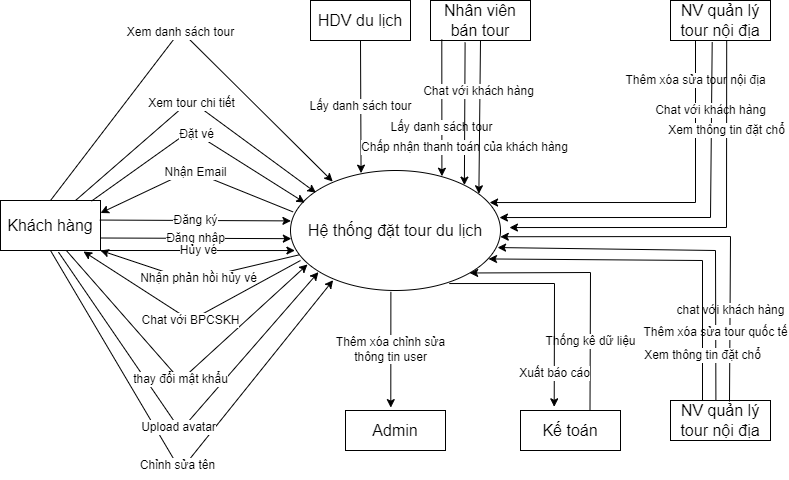
\includegraphics[width = 1\linewidth]{figures/DFDsContext.png}
    \caption{Context diagram}
    \label{fig:example_1}
\end{figure}

\vspace{10cm}

\subsubsection{Level-1 diagram}
\subsubsection{Level-0 diagram}

\textTo{Sơ đồ thể hiện các luồng chức năng một cách chi tiết nhất}
\vspace{3cm}

\begin{figure}[ht]
    \centering
    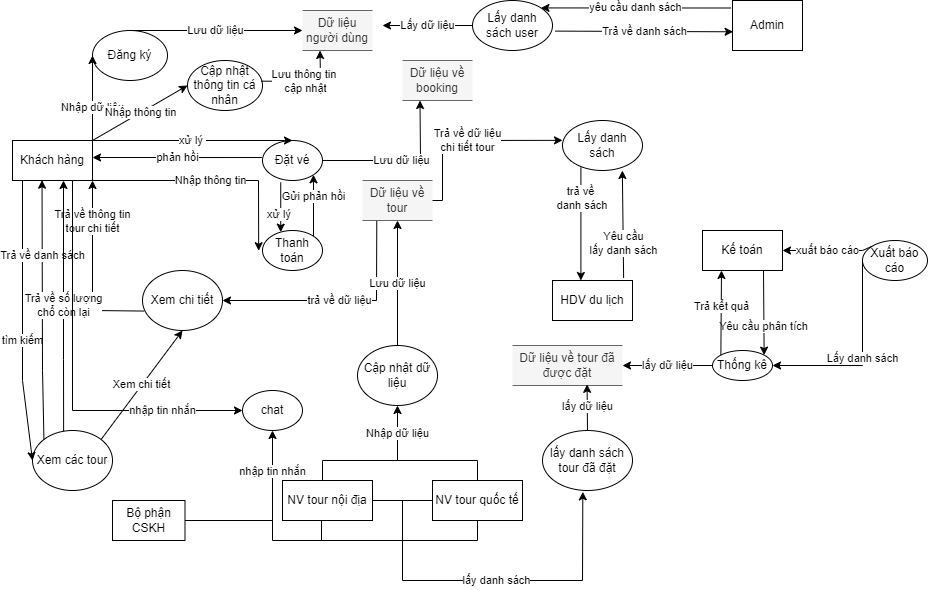
\includegraphics[width = 1.2\linewidth]{figures/DFD-level0.png}
    \caption{Sơ đồ Level-0 diagramt.}
    \label{fig:example_1}
\end{figure}

% \subsubsection{Level-1 diagram}

% \vspace{10cm}
\subsection{Lượt đồ ERD}

\vspace{7cm}

\begin{figure}[ht]
    \centering
    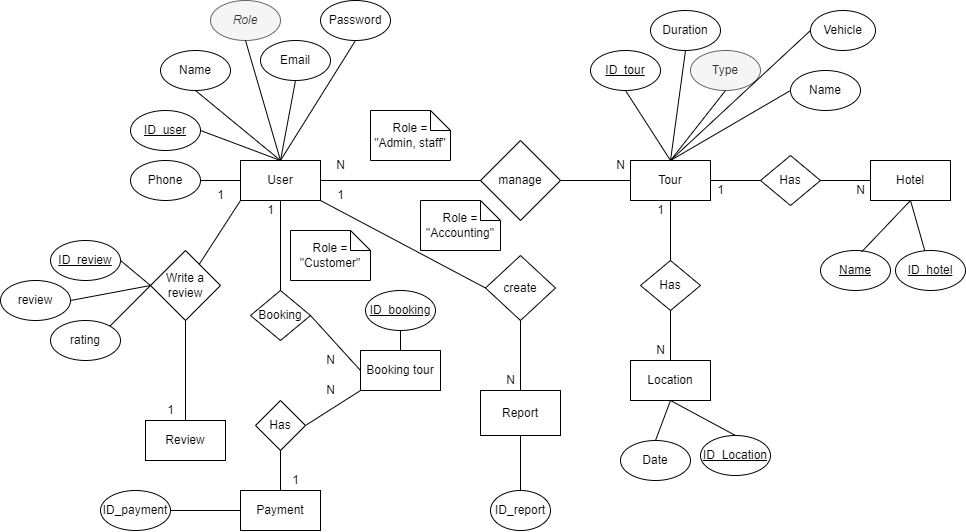
\includegraphics[width = 1.2\linewidth]{figures/ERD.png}
    \caption{Sơ đồ ERD.}
    \label{fig:example_1}
\end{figure}

\subsection{Lượt đồ EERD}

\vspace{7cm}

\begin{figure}[ht]
    \centering
    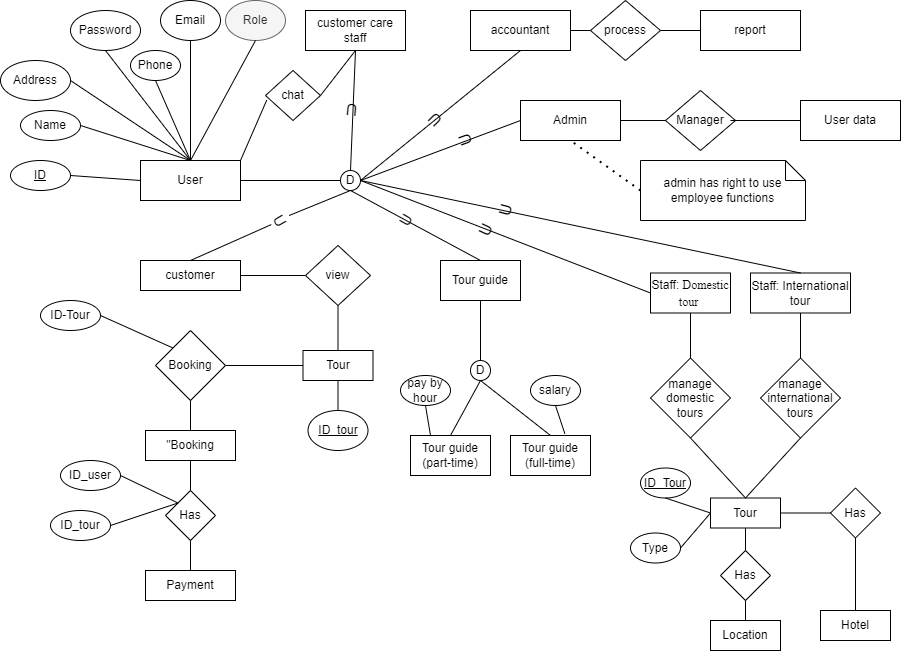
\includegraphics[width = 1.2\linewidth]{figures/EERD.png}
    \caption{Sơ đồ EERD.}
    \label{fig:example_1}
\end{figure}

% \vspace{10cm}
\section{HIỆN THỰC HỆ THỐNG}

\subsection{Framework lập trình}

\textTo{Backend: ExpressJS}

\textTo{Fontend: Pug template (HTML + CSS + JS)}

\textTo{Database: MongoDB}

\subsection{Database}

\vspace{2cm}

\begin{figure}[ht]
    \centering
    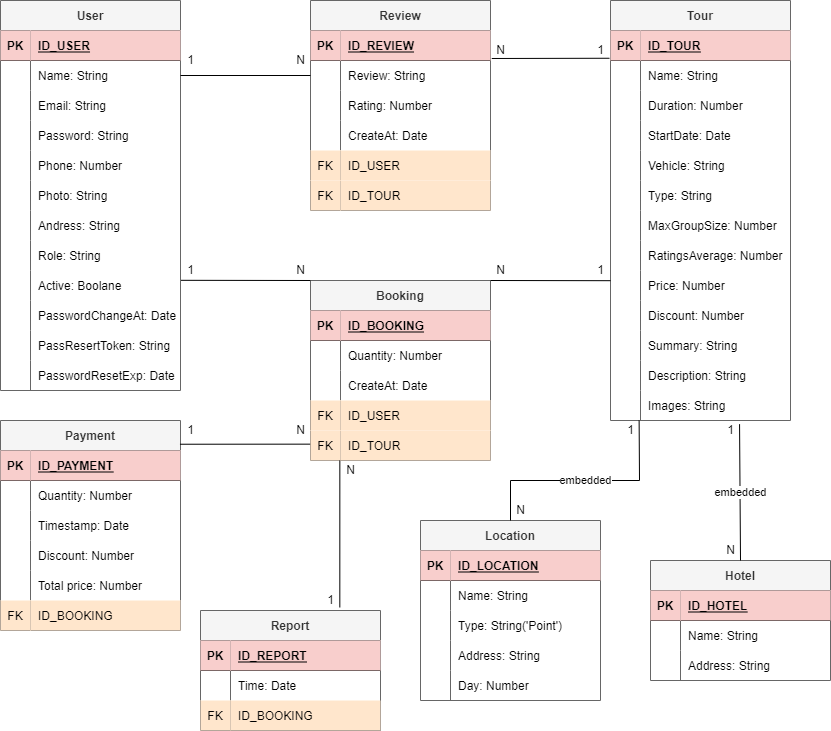
\includegraphics[width = 1.1\linewidth]{figures/ddp.png}
    \caption{Database.}
    \label{fig:example_1}
\end{figure}

\vspace{10cm}
\subsection{Security}

\subsubsection{Compromised database}

\begin{itemize}
\item Mã hóa mật khẩu với salt và hash (bcrypt)
\item Mã hóa password reset tokens (SHA 256)
\end{itemize}

\subsubsection{Brute force attacks}

( Hacker có thể cố gắng đoán password bằng cách thử hàng triệu password ngẫu nhiên)

\begin{itemize}
\item Sử dụng bcrypt
\item Triển khai rate limiting (express-rate-limit) – đặt giới hạn request cho 1 ID nhất định
\item Triển khai maximum login attemps (đặt móc thời gian nếu user nhập sai 10 lần)
\end{itemize}

\subsubsection{Cross-site scripting (xss) attacks }
( Nơi hacker cố gắng đưa các script độc vào web – có thể đọc local storage )

\begin{itemize}
\item Lưu JWT ở  HTTPOnly cookies
( không nên lưu JWT ở local storage => nên lưu vào HTTP-cookie => trình duyệt nhận và gửi cookie nhưng cookie settings không thể truy cập và sửa đổi)
\item Santitize user input data
\item Set special HTTP headers (helmet package)
\end{itemize}

\subsubsection{Denial-of-service (dos) attack}

Hacker gửi quá nhiều request khiến server bị break down

\begin{itemize}
\item Triển khai rate limiting (express-rate-limit)
\item Limit body payload (in body-parser) => giới hạn dữ liệu được gửi lên server
\end{itemize}

\subsubsection{NOSQL query injection}

\begin{itemize}
\item Use Mongoose for MongoDB
\item Santitize user input data
\end{itemize}


\subsubsection{Đề xuất các phương pháp khác}

\begin{enumerate}
\item Luôn luôn sử dụng HTTPs (nếu không hacker có thể vào ăn cắp JWT)
\item Create random password reset tokens with expiry dates (hiệu quả)
\item Từ chối  JWT cũ sau khi thay đổi passowrd
\item Không gửi lỗi quá chi tiết cho user (dễ khai thác lỗ hỗng)
\item Triển khai blacklist các JWT không đáng tin cậy
\item Xác nhận qua email khi tạo tài khoản 
\end{enumerate}





\section{DEMO}

\addcontentsline{lof}{figure}{Demo}

\textbf{Nghiệp vụ của khách hàng:}

\textTo{Khách hàng truy cập website sẽ hiển thị danh sách các tour}

\begin{figure}[ht]
    \centering
    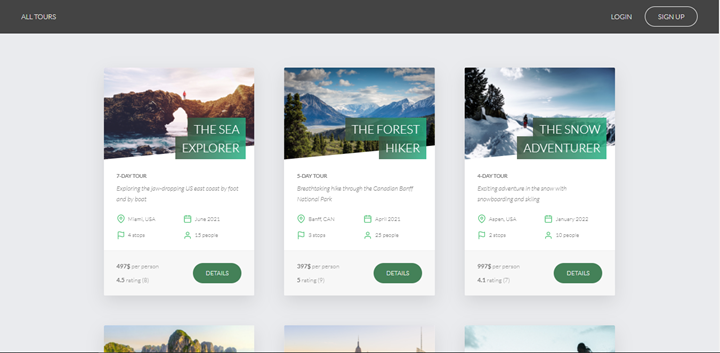
\includegraphics[width = 1.2\linewidth]{figures/demo/1.png}
    \caption{Hình ảnh danh sách tour.}
    \label{fig:example_1}
\end{figure}

\vspace{10cm}

\textTo{Khách hàng chọn xem chi tiết tour}

\begin{figure}[ht]
    \centering
    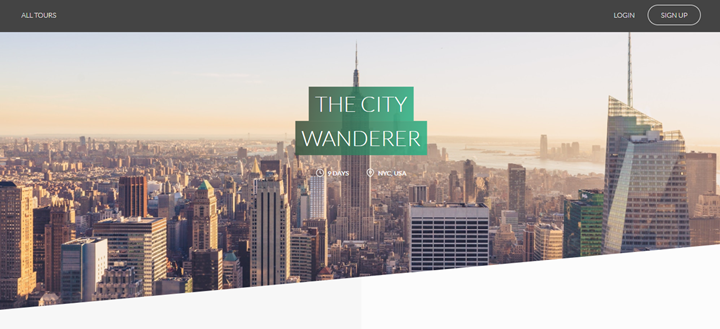
\includegraphics[width = 1.2\linewidth]{figures/demo/2.png}
    \label{fig:example_1}
\end{figure}
\begin{figure}[ht]
    \centering
    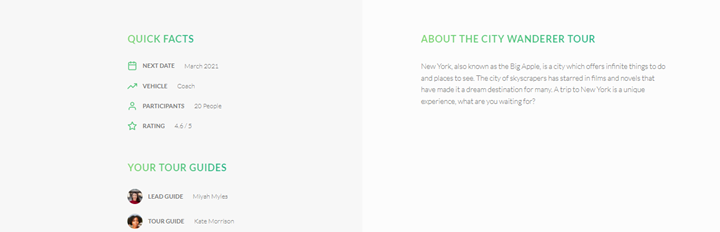
\includegraphics[width = 1.2\linewidth]{figures/demo/3.png}
    \caption{Chi tiết tour.}
    \label{fig:example_1}
\end{figure}

\vspace{15cm}

\textTo{Xem bản đồ chi tiết về ngày, nơi đến.}


\begin{figure}[ht]
    \centering
    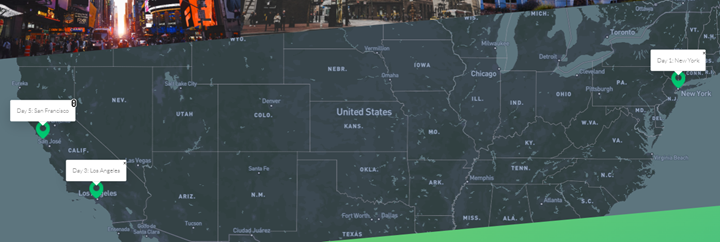
\includegraphics[width = 1.2\linewidth]{figures/demo/bando.png}
    \caption{Bản đồ chi tiết về ngày và nơi đến.}
    \label{fig:example_1}
\end{figure}

\textTo{Xem đánh giá từ các người đã đi tour này}

\begin{figure}[ht]
    \centering
    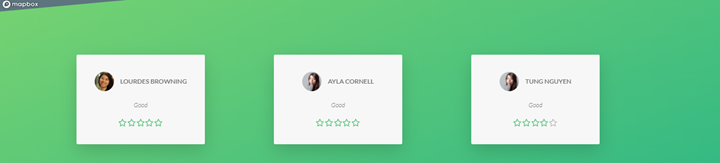
\includegraphics[width = 1.2\linewidth]{figures/demo/5.png}
    \caption{Xem đánh giá từ các người đã đi tour này.}
    \label{fig:example_1}
\end{figure}

\vspace{10cm}

\textTo{Khách hàng sẽ thấy button đặt tour phía dưới cùng, Khách hàng sẽ được yêu cầu đăng nhập để đặt tour}

\begin{figure}[ht]
    \centering
    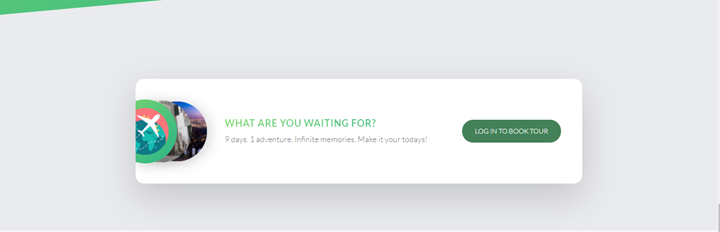
\includegraphics[width = 1.2\linewidth]{figures/demo/6.png}
    \caption{Button đặt tour.}
    \label{fig:example_1}
\end{figure}

\textTo{Nếu khách hàng chưa có tài khoản thì sẽ được phép đăng ký tài khoản mới}

\begin{figure}[ht]
    \centering
    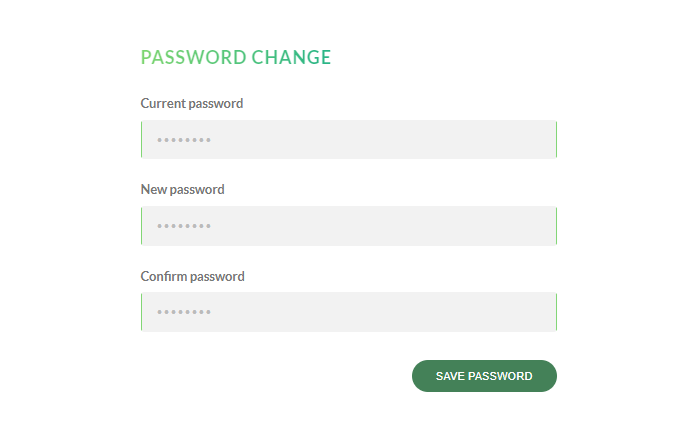
\includegraphics[width = 1\linewidth]{figures/demo/11.png}
    \caption{Đăng ký tài khoảng mới.}
    \label{fig:example_1}
\end{figure}

\vspace{10cm}

\textTo{Sau khi đăng ký thành công thì Khách hàng sẽ nhận được thư qua gmail}

\begin{figure}[ht]
    \centering
    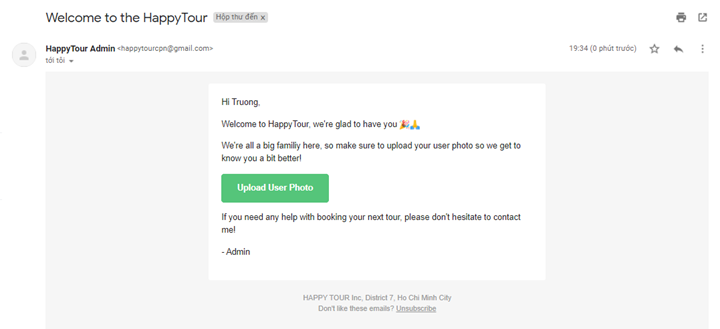
\includegraphics[width = 1\linewidth]{figures/demo/mail.png}
    \caption{Mail xác nhận.}
    \label{fig:example_1}
\end{figure}

\begin{figure}[ht]
    \centering
    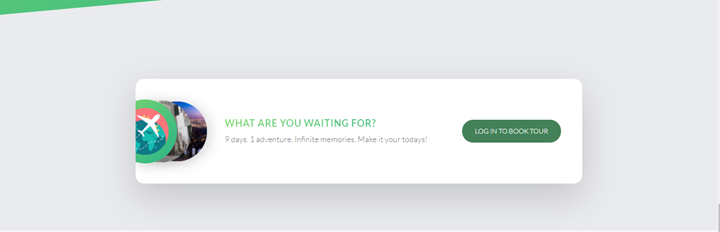
\includegraphics[width = 1\linewidth]{figures/demo/6.png}
    \caption{Button đăng ký tài khoản.}
    \label{fig:example_1}
\end{figure}

\textTo{Sau khi click vào button sẽ chuyển đến trang thanh toán cho khách hàng}

\vspace{10cm}

\textTo{Các thông tin thanh toán được hiển thị đầy đủ}

\begin{figure}[ht]
    \centering
    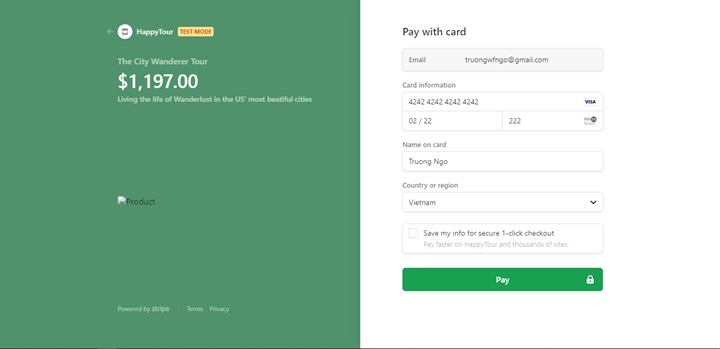
\includegraphics[width = 1\linewidth]{figures/demo/pay.png}
    \caption{Trang thanh toán.}
    \label{fig:example_1}
\end{figure}

\textTo{Phía hê thống sẽ tiếp nhận và xử lý gửi hóa đơn cho khách hàng qua email}

\begin{figure}[ht]
    \centering
    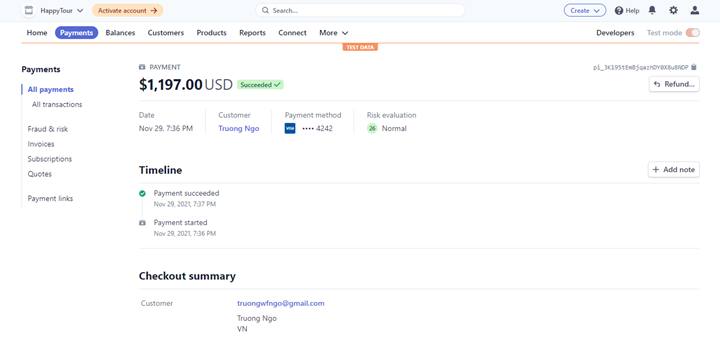
\includegraphics[width = 1\linewidth]{figures/demo/pay1.png}
    \caption{Trang thanh toán.}
    \label{fig:example_1}
\end{figure}

\textTo{Các chức năng ở phần hệ thống quản lí đã làm được hết các API chưa hoành thành bên fronEnd để dựng trang admin}

\begin{figure}[ht]
    \centering
    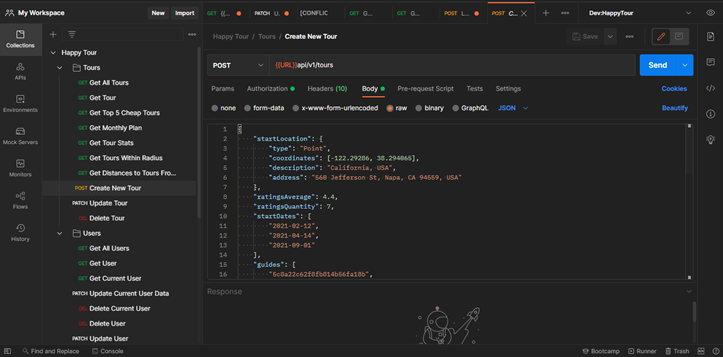
\includegraphics[width = 1\linewidth]{figures/demo/api.png}
    \caption{Trang thanh toán.}
    \label{fig:example_1}
\end{figure}

\vspace{10cm}

\section{Kết luận}

Báo Cáo đã đạt được các yêu cầu cần thiết
\subsection{Phần đồ án:}
\begin{itemize}
\item Hoàn thành các chức năng về nghiệp vụ của khách hàng đã dựng lên web thành công
\item Các chức năng quản lí nội bộ vẫn ở mức API (hoàn thành) chưa triển khai lên trang admin
\item Thiếu các chức năng của kế toán và bộ phận CSKH
\end{itemize}




\input{sections/References}




%If you came here because you want your references in a new page, uncomment the following line

%\clearpage % If you want the references in a separate page
\bibliography{bibliography}


\clearpage % If you want the appendix in a separate page


\begin{enumerate}
\item Alan Dennis, Barbara Haley Wixom, Roberta M. Roth, [2018], Systems Analysis and Design, 7th Edition, John Wiley & Sons, Inc., USA\cite{yonatan2018managing}
\item Eric Jendrock, Ricardo Cervera-Navarro, Ian Evans, Devika Gollapudi, Kim Haase, William Markito, Chinmayee Srivathsa, [2014], Java Platform, Enterprise Edition: The Java EE Tutorial E39031-01, Oracle, United State\cite{elmasri2000fundamentals}
\item Ramez Elmasri, Shamkant B. Navathe, [2016], Fundamentals of Database Systems, 7th Edition, Pearson, USA
\end{enumerate}\cite{xkcd}



\end{document}
